\documentclass[letterpaper]{article}
\usepackage[submission]{aaai2027}
\usepackage{graphicx}
\usepackage{amsmath}
\usepackage{amssymb}
\usepackage{booktabs}
\frenchspacing

\pdfinfo{
/TemplateVersion (2027.1)
}

\title{Supplementary Material: From Fault Evidence to Control Consequences}
\author{Anonymous submission}
\affiliations{}
\date{}

\begin{document}
\maketitle

\section{Complete Fault Protocol}

\begin{table}[t]
\centering
\scriptsize
\setlength{\tabcolsep}{3.1pt}
\begin{tabular}{@{}lccccc@{}}
\toprule
Operator & Target & Train & Det.\ select & Gate tune & Test\\
\midrule
Insole missing & insole & yes & yes & yes & yes\\
Encoder dropout & encoders & yes & yes & yes & yes\\
IMU bias ramp & shank IMU & yes & yes & no & yes\\
Packet loss & all groups & yes & yes & yes & yes\\
Stuck IMU & foot IMU & yes & no & no & yes\\
Sensor delay & all groups & yes & yes & yes & yes\\
\midrule
Burst loss & all groups & no & no & no & yes\\
Partial-channel loss & all groups & no & no & no & yes\\
Delay jitter & all groups & no & no & no & yes\\
\bottomrule
\end{tabular}
\caption{Exact role of each evaluated operator. ``Det.\ select'' denotes
validation-only subset selection, not test evaluation. The final three rows are
held-out operators within the packet-loss and delay families; they are not
claimed to represent open-set hardware faults. IMU bias and stuck IMU were
excluded from gate tuning by the archived configuration.}
\label{tab:fault-protocol}
\end{table}

Every injected fault occupies the full 768-sample window and therefore has a
window-constant label. The protocol tests steady-state corruption
discrimination, not onset latency, recovery, transient faults, or simultaneous
faults. Clean and corrupted test scenarios reuse the same split-level source
corpus, enabling the aggregate clean-adjusted contrast below.

\newpage
\begin{figure*}[t]
\centering
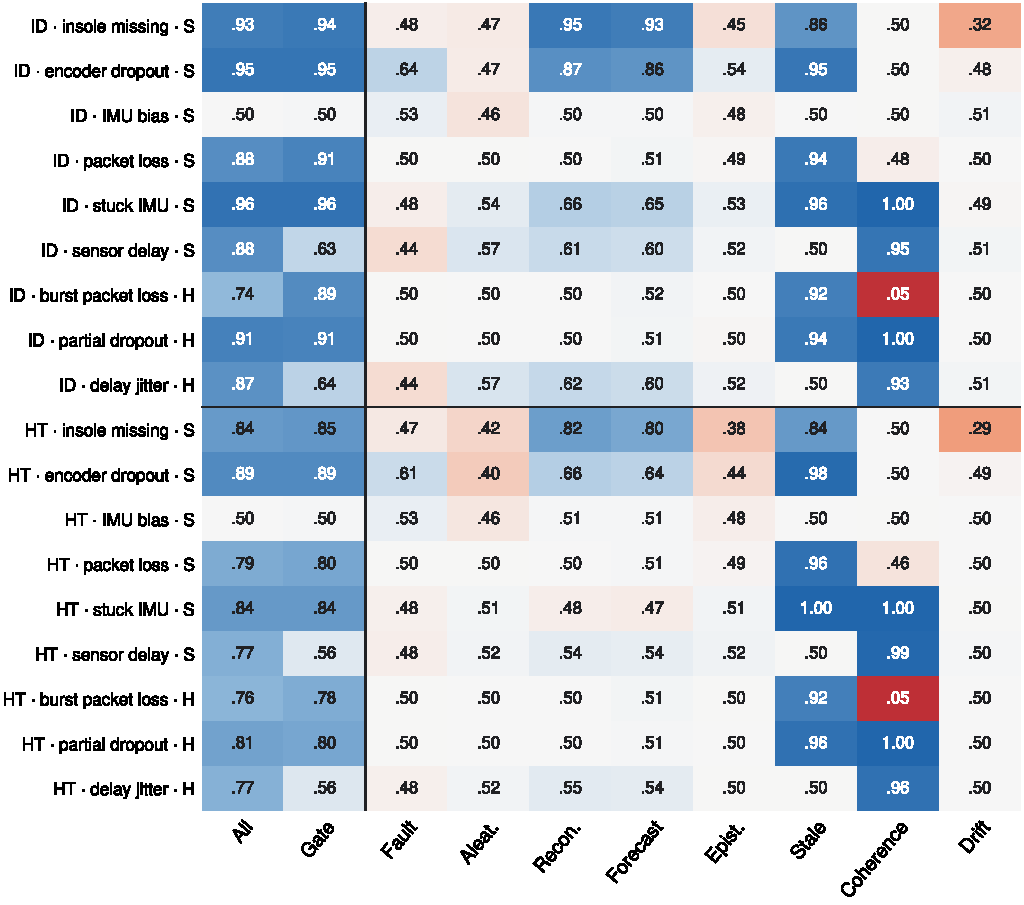
\includegraphics[width=\textwidth]{figures/fig_detection_full.pdf}
\caption{Complete split-specific detectability matrix, mean over seeds 7, 13,
and 23. No evaluated operator or candidate channel is omitted. ID and HT denote
in-distribution and training-held-out tasks; S/H denote training-seen and
held-out operators. ``All'' and ``Gate'' are validation-selected evaluation
subsets, not the actual timestep gate, which uses all available gate channels.
Color diverges about chance (AUROC 0.5).}
\label{fig:detection-full}
\end{figure*}

\section{Metric Identity and Clean-Adjusted Contrast}

For the evaluated gate, $u_n^{g}=g_nu_n^0$ with $g_n\in[0,1]$. Hence
\[
\mathbb{I}[u_n^{g}\tau_n^\star<0]
=\mathbb{I}[u_n^0\tau_n^\star<0]\mathbb{I}[g_n>0],
\]
so the wrong-direction fraction cannot increase and changes only at exact
shutdowns. The archived clean/fault wrong-direction non-increase checks are
therefore identities, not active constraints. The main paper accordingly makes
the continuously responsive $X_{\mathrm{opp}}$ primary and retains the count
only as a hard-shutdown diagnostic.

Within each seed and task split, we subtract the clean gate change from every
fault-scenario change and then macro-average the nine faults. The raw fault
change, matched clean change, and clean-adjusted change are respectively
$-0.736\pm0.067$, $-0.397\pm0.043$, and $-0.339\pm0.098$ percentage points for
the wrong-direction fraction. For $X_{\mathrm{opp}}$ they are
$-0.0114\pm0.0020$, $-0.0044\pm0.0009$, and $-0.0070\pm0.0015$
$(\mathrm{Nm/kg})^2\mathrm{s}$. These standard deviations are across the three
training seeds. This is a scenario-aggregate matched contrast, not a
window-level paired confidence interval.

\section{Ordered Component Attribution}

\begin{figure*}[t]
\centering
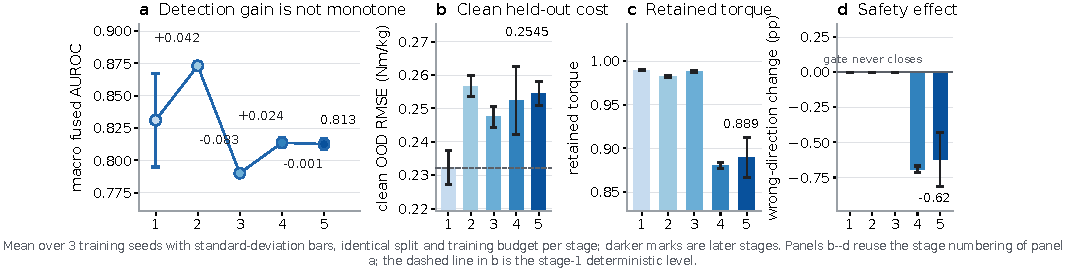
\includegraphics[width=\textwidth]{figures/fig_ablation_summary.pdf}
\caption{Ordered component attribution on a fixed split and training budget.
Stages 1--5 are the deterministic non-augmented TCN, fault augmentation,
probabilistic regression, reconstruction, and forecasting. Panels (b)--(d)
reuse that numbering. (a) Macro Detector-all AUROC per stage, with signed
annotations for adjacent, seed-paired changes. (b) Clean training-held-out-task
RMSE; the dashed rule is the deterministic stage-1 level. (c) Retained aligned
torque and (d) wrong-direction change in percentage points under each stage's
own validation-selected gate, macro-averaged over the fixed fault set. Means
are over seeds 7, 13, and 23; bars are cross-seed standard deviations.}
\label{fig:ablation-supp}
\end{figure*}

Detector-all is shown because each stage's evaluation subset is selected within
that candidate pool. Detector-gate is also evaluated for every stage. The
reconstruction step is the only sign disagreement: its adjacent change is
$+0.024\pm0.004$ for Detector-all and $-0.013\pm0.002$ for Detector-gate,
because the residual displaces coherence without matching it on delay faults.
Stages 1--3 select a deadband that their test risks never exceed, so their
wrong-direction changes are exactly zero rather than rounded small values.

\section{Severity Extremes and Subject Transfer}

\begin{figure}[t]
\centering
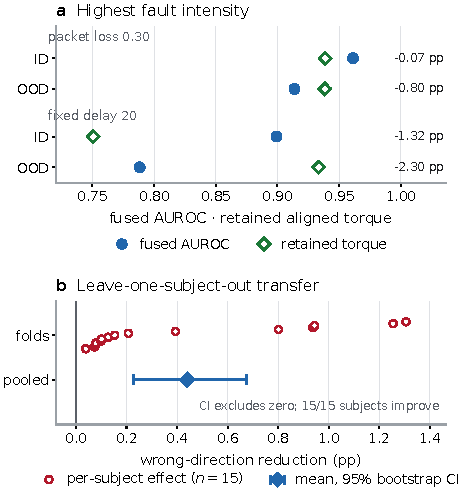
\includegraphics[width=\columnwidth]{figures/fig_stress_transfer.pdf}
\caption{Severity extremes and subject transfer. (a) Packet-loss rate $0.30$
and fixed delay $20$ samples ($100$ ms). Filled circles are Detector-all
AUROC, open circles Detector-gate AUROC, and open diamonds aligned-assistance
retention; labels give wrong-direction changes. Points are means over three
training seeds and horizontal bars are cross-seed standard deviations. (b)
Each circle is one leave-one-subject-out fold; the diamond is the mean with its
$95\%$ percentile-bootstrap interval over $15$ folds ($10{,}000$ resamples,
bootstrap seed 0).}
\label{fig:stress-supp}
\end{figure}

The leave-one-subject-out effect for a participant is the reduction in
wrong-direction fraction, first macro-averaged over nine faults and the two
task splits. The resulting 15 values have mean $0.44$ percentage points,
between-participant standard deviation $0.47$, range $0.04$--$1.31$, and
$95\%$ percentile-bootstrap interval $[0.23,0.67]$. All 15 values are positive.
This fold-level interval, rather than the variation over three training seeds,
supports the manuscript's primary uncertainty statement.

\clearpage
\section{Reproduction Notes}

The submission package contains the official AAAI reproducibility checklist
and a separate anonymous reproduction note. It also includes the scripts that
construct the aggregate tables and figures from archived per-run JSON reports.
The legacy JSON field names \texttt{wrong\_energy} and
\texttt{mean\_abs\_jerk} are compatibility aliases: the corresponding
quantities are the opposition-weighted torque-product integral in
$(\mathrm{Nm/kg})^2\mathrm{s}$ and mean absolute torque rate in
Nm\,kg$^{-1}$\,s$^{-1}$, respectively.

Main training uses batch size 64, 20 epochs, AdamW with learning rate
$10^{-3}$ and weight decay $10^{-4}$, gradient-norm clipping at 5, 768-sample
windows at stride 384, at most four windows per trial, and no learning-rate
schedule or early stopping. With the configured negative
\texttt{clean\_sample\_prob}, clean and each of the six training faults are
sampled uniformly. The checkpoint minimizes clean-validation
$\mathrm{RMSE}+0.02\,\mathrm{coverage\ ECE}$ over epochs.

The staleness statistic uses threshold $10^{-3}$ and a 25-sample trailing
window; coherence uses a 32-sample trailing window and clamps each rolling
variance below at $10^{-8}$. The main suite uses 10 MC-dropout passes.
Hip/knee moment-to-torque scales are $(0.20,0.15)$, delays are $(10,0)$ samples,
the low-pass cutoff is 6 Hz, and saturation is 0.45 Nm/kg. Coverage ECE uses
nominal levels 0.50, 0.68, 0.90, and 0.95. $X_{\mathrm{opp}}$ is summed over
the evaluated samples and is not normalized by recording duration; all paired
comparisons use identical samples. Each LOSO fold uses training seed 7 and the
preceding participant as validation, so the 15 fitted training sets overlap.

\end{document}
